\documentclass[11pt]{article}
\usepackage{framed}

\usepackage{fullpage}
\usepackage{amsmath}
\usepackage{listings}
\usepackage{tikz}
\usepackage{amsmath}
\usepackage{wrapfig}
\usepackage{float}
\lstset{language=C}
\begin{document}

\title{Survivability of ICU Patients with Severe Sepsis/Septic Shock}
\author{Jeremy B. Crowe - crowe.jb@gmail.com}
\maketitle

\section{Domain Background}
\subsection{Overview}
Sepsis is a serious, life-threatening condition that is partially responsible for 6\%  of all deaths in the United States~\cite{cdc}. A septic condition is highly variable in nature. A patient may arrive at the ICU with sepsis or may be diagnosed during the stay. There is no diagnostic test to confirm or deny the existence of such a condition in a patient. It is diagnosed based on the clinical judgment of the physician. Regardless of the cause, the speed at which treatment is administered and the types of treatments are critical in stabilizing a patients blood pressure, body temperature, eliminate infection, and keep cardiac output stable. Due to the variable, and difficult nature of the condition a machine learning approach may be able to aid in predicting the severity or survivability of the condition and the effectiveness of potential treatments.

A septic condition is caused by an overwhelming immune response to an infection. White blood cells release an array of chemicals to fight the infection which triggers systemic inflammation, vasodilation, increased permeability of vessels, and intracellular fluid build up. These ``leaky vessels'' deplete the body of coagulation factors. The increased fluid build-up and decreased blood pressure result in a lack of oxygenation of tissue, known as shock.

If sepsis is not treated quickly or with enough direct care, multiple organ dysfunction can occur which can result in kidney failure, liver failure, heart failure, acute respiratory distress, etc. The speed at which treatment is administered and types of treatments are directly correlated with the survivability of this severe condition. The speed of treatment has been found to be more important than the age of the patient~\cite{survival2}. Each hour of delay in antimicrobial administration over the initial 6 hours is associated with an average decrease in the survival rate of 7.6\%~\cite{survival}.

Certain treatments may be highly effective, therefore it is important to pay special attention to several things: the type of infection and type of antibiotics used, the blood pressure and whether or not vasopressors were used, the correct amount of IV fluid provided to the patient. The correct type of antibiotic and appropriate administering of vasopressors can reduce the chance of organ failure and mortality greatly~\cite{pressors}.


\subsection{Problem}

A predictive model would be highly useful for ICU staff and physicians. It would aid in prioritizing patients that are considered ``high risk'' and as a simple way to stratify patients in clinical research. 

Upon patient admittance and initial blood and microbiology tests patient survivability will be classified over a 30 day period. While survival rates are available long after 30 days, this is the most critical period for surviving a condition such as sepsis/septic shock. 

Test results and vitals from the first 24 hours in the ICU will be used for consideration. Several class features will be considered: gender, bacterial culture classification, antibiotic treatment, etc. Several continuous features will also be considered: blood urea nitrogen levels, age, blood PH, blood lactate levels, creatinine levels, blood pressure, etc.

The survivability of sepsis is strongly correlated with the speed of treatment, the age of the patient, type of infection, and the general state of the condition. The state of the condition can be measured in a variety of ways. Respiratory rate, blood pressure, creatinine (kidneys failing), and lactate levels(anaerobic cellular respiration) strongly suggest the current stage of the condition. Upon arrival, these measurements can be used to classify a patient into a binary survival group.

\subsection{Metrics}
The metric that will be used to gauge the prediction quality is the standard classification accuracy. Classification accuracy is the total number of true positives and true negatives out of all datapoints. It is defined as follows:

\[ \text{accuracy} = \frac{\text{true positives} + \text{true negatives}} {\text{total datapoints}} \]



This metric is used because the low survivability of sepsis. False positives and false negatives erode the usefulness of further patient studies.

\textbf{Caveat:} Accuracy is not enough in a real world application if the outcome affects human life. Accuracy weighs misclassifications evenly. This is useful when looking at a problem mathematically. Consider the following however: A patient is given a high probability that their cancer is in remission and no further treatment is given. It was a false negative classification and the patient dies. This is much more important to consider than a false positive. Therefore these results are only used in stratifying patients for further studies, not as a real time aid in patient treatment.

Many patients die of sepsis however, around 30\%. Due to this high ratio and the intended problem of stratifying patients for future studies, an accuracy score is useful. If used in a different application, it may be useful to select a model with lower accuracy that ensures very low rates of false negatives, a more dangerous false prediction.

\section{Analysis}
\subsection{Data Exploration}
For this study, the MIMIC-III dataset(https://mimic.physionet.org/) will be used. This dataset is freely accessible and suggested for use by Udacity. More than 40,000 individual patient entries will be utilized. 1184 patients were admitted with sepsis and thousands more diagnosed by the end of their stay. Most of the focus will be put on the patients admitted with sepsis since there is an associated time of admittance that will aid in finding more effective treatments.

Once input into a Postgres database, there are 20 tables with patient information and 5 dictionary lookup tables. Much of the data is difficult to process due to lack of standardization across multiple source databases(CareVue and MetaVision). Most of the useful information with datetime information associated with it is available in the following tables: admissions, patients, labevents, microbiology events

\begin{enumerate}
	\item \textbf{admissions}: Contains information related to a patient's admission. This information includes their hospital stay id, insurance type, date of admission, and suspected diagnosis/condition.
	\item \textbf{patients}: Patient information such as date of birth, gender, hospital stay id, etc. 
	\item \textbf{labevents}: Patient lab events with datetime associated with the measurement. This includes information such as creatinine levels.
	\item \textbf{microbiologyevents}: Patient microbiology tests with datetime associated with the result. This includes tests for infections and resulting prescription.
\end{enumerate}

Due to the size, variability, and nature of ICU care much of this data must be explored for feasibility in a machine learning model. A good example is blood pressure. While in the MetaVision database, it was standardized with mm/Hg, in the Carevue database that was not the case. It makes the data less useful since information is not standard across different patient entries.

\subsection{Exploratory Visualizations}
The basic patient information housed within the \textbf{Admissions} table has some potentially useful information. Combining their admission date with their dob we can calculate their age(except patients over 89 due to HIPAA regulations). The visualization of survivability with age is as follows can be observed in \textbf{figure 1}.

\begin{wrapfigure}{r}{0.5\textwidth}
	\begin{center}
		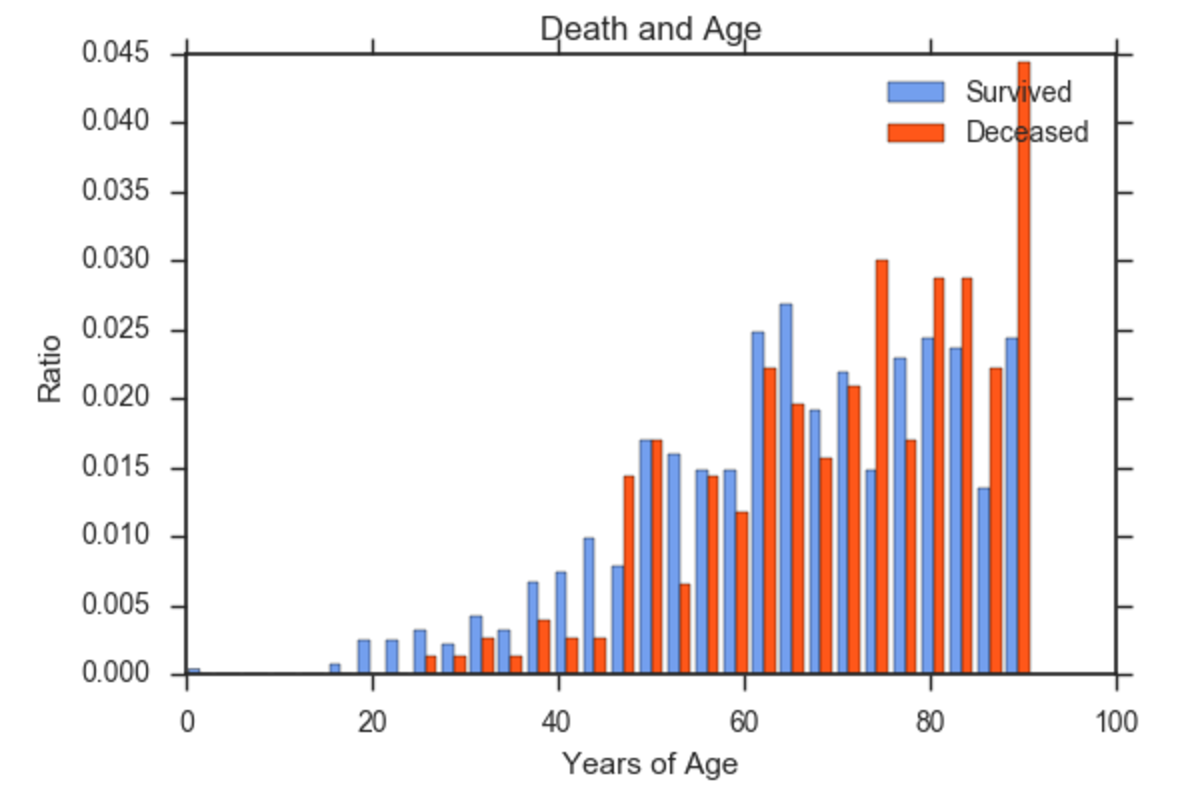
\includegraphics[width=0.48\textwidth]{age.png}
	\end{center}
	\caption{Age Breakdown}
\end{wrapfigure}

There is a somewhat noticeable trend in \textbf{figure 1} with regards to age and survivability of sepsis but it doesn't appear to be anything that an algorithm could rely on strongly. It is important to discover some other useful features.

It may be useful to look at the initial blood tests for feature correlation. Observing all of these blood tests that are correlated with sepsis, the following were had enough datapoints to be useful: bicarbonate, INR, MCH, AST, alkaline phosphatase, PH, creatinine, platelet, PT, PTT, lymphocytes, RBCDW, calcium, neutrophils, glucose, hematocrit, hemoglobin, lactate, BUN, age.

Looking at the feature correlation in \textbf{figure 2} gives a better understanding of how the features are correlated with one another as well as which features have a strong or negative correlation to the survivability of sepsis.




There appear to be a few values with very strong correlation such as PTT and INR. PTT, PT, and INR are all used to test for clotting factors in blood so this result is logical. This also means that these features could probably be compressed into fewer dimensions.

\begin{wrapfigure}{l}{0.70\textwidth}
	\begin{center}
		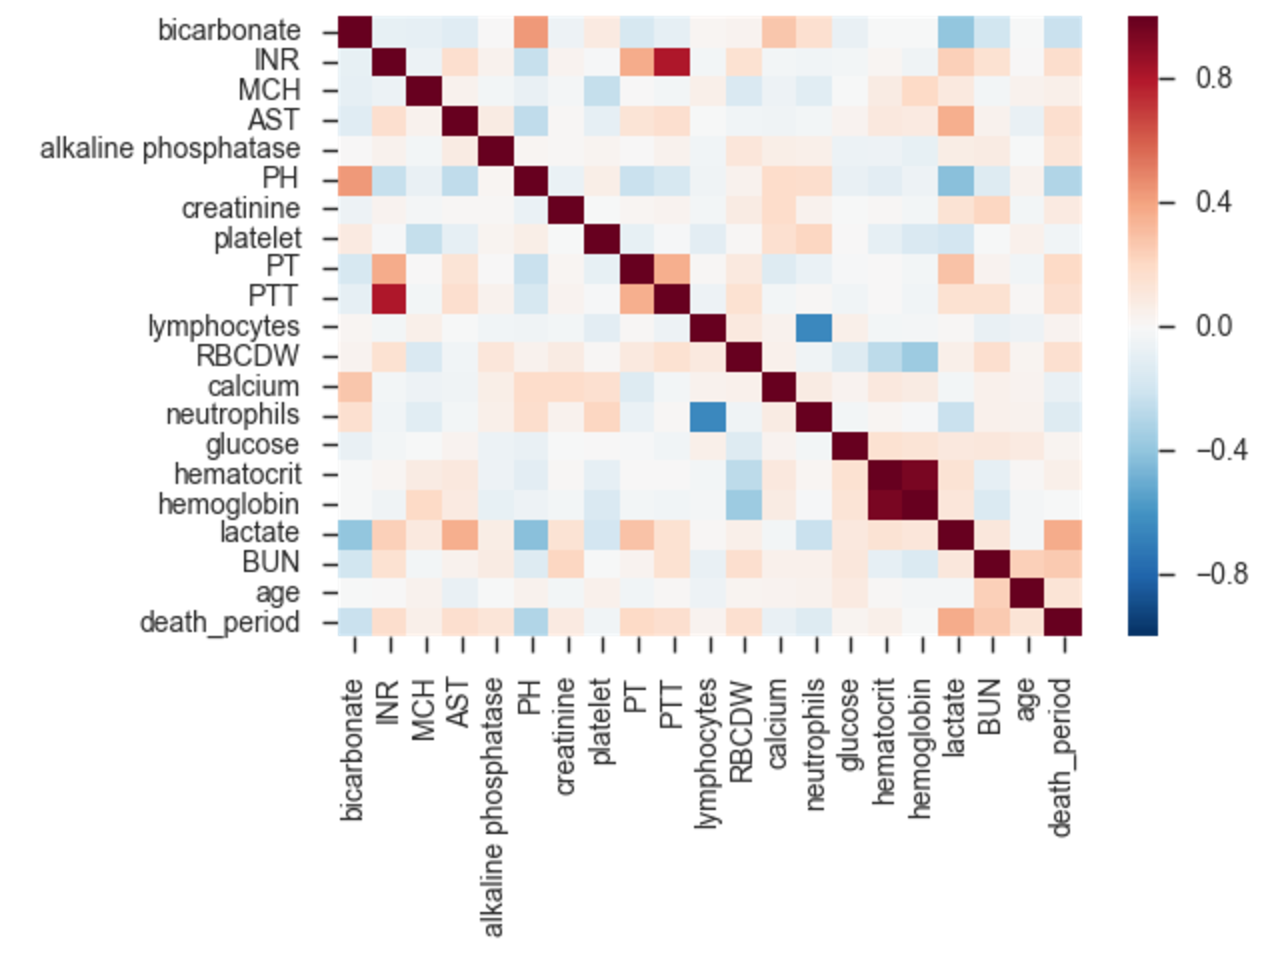
\includegraphics[width=0.68\textwidth]{feature_correlation.png}
	\end{center}
	\caption{Patient Vitals Correlation}
\end{wrapfigure}

Within the 30 day period of mortality, there are none with a positive or negative correlation over +/-0.4 however there are some useful features to consider. Lactate is relatively strongly correlated with ~0.38 with blood urea nitrogen(BUN), and PH not far behind. Lactate is an indication of shock, since lactate is produced by cells that are note receiving enough oxygen. PH is a byproduct of the acidic lactate in the patients blood hence the correlation. Blood urea nitrogen is an indication that the kidneys are failing to process the excess urea in the blood. This can indicate potential kidney damage or failure. All of these are much more useful than age, which is a good sign for our ability to predict.

\begin{wrapfigure}{r}{0.50\textwidth}
	\begin{center}
		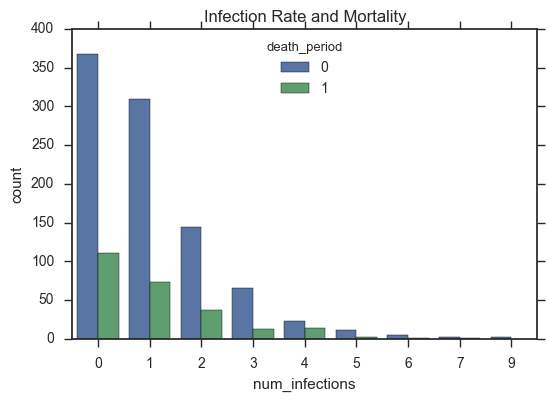
\includegraphics[width=0.48\textwidth]{bio_graph.png}
	\end{center}
	\caption{Infection Count and Mortality}
\end{wrapfigure}

Finally considering microbiology events. Every infection type is taken and the correlation considered. Though the assumption might be made that infection is strongly correlated with the survivability of sepsis, it is important to note that once a patient is septic, the infection type plays little role. Let us look at number of infections and survivability in \textbf{figure 3}.

There appears to be very little correlation after further observation between survivability and number of infections. With the majority of patients not having an infection discovered within the first 24 hours. Due to this lack of information, the infection type is likely not useful. 

These visualizations give some useful insights into the data. One of these insights is that there is nothing that strongly indicates a patient will or will not survive sepsis. Many independent features must be taken into consideration and trends found. Due to this nature of the data, a neural network, or an ensemble technique like adaptive boosting or extreme gradient boosting may prove useful. 



\subsection{Algorithms and Techniques}
Four different classifiers will be compared for their accuracy score. These classifiers are the following:

\begin{enumerate}
	\item \textbf{Random Forest:} Random forests are a highly useful ensemble method that is one of the single most accurate learning algorithms right out of the box. It provides a useful analysis as to feature importance as well. It is relatively fast to train but does have limitations on predictions, though these limitations are not tested with this use case. It is also known to seldom overfit to data.
	
	Random forests do have their down sides however. Like most other algorithms that are to be used here, it falls into the black box domain. It performs better the larger the dataset, and this dataset is not terribly large at around 1200 entries. Random forests are biased in multiclass problems toward more frequent classes. In this classification problem, patient survival is around 70\% of cases. This could affect the results of this algorithm.
	
	\item \textbf{Adaptive Boosting:} Adaboost is another fantastic ensemble method. It is notorious for not overfitting to data. It is quite flexble due to its ability to leverage any base estimator works best in a certain situation. Adaboost itself has few parameters to tweak to increase performance so it works relatively well right out of the box.
	
	While Adaboost is one of my favorite algorithms so far, it does have some pretty strong weaknesses. It is most often always not the best in class predictor. There typically are more accurate classifier options on the table. It is also sensitive to noisy data as well as outliers. This is similar to Random Forests. The reason I included both of these ensemble techniques is because I wanted to compare their output to classifiers known to be better at handling noisy data. These are great classifiers but are unlikely to be the most accurate.
	
	\item \textbf{Neural Network:} Neural networks are an incredibly powerful machine learning algorithm. They can approximate any nonlinear function, highly customizable, and robust to outliers. With these features, it is possible to create a highly accurate predictor of the data but it is important to take into consideration the weaknesses of neural networks as well.
	
	Neural networks, while powerful, have some pretty strong weaknesses. They are difficult to set up and difficult to tune because of the number of parameters. It is also necessary to decide on the architecture of the network yourself. It is not nearly as simple to set up as the previous examples. It is also quite easy to overfit data using neural networks. Without restraint they have a strong affinity to fit to noise in the data. Due to the nature of this dataset it will be a important task to keep this algorithm in reign to prevent overfitting.
	
	\item \textbf{Extreme Gradient Boosting} XGBoost is an optimized distributed gradient boosting library. Gradient boosting in general is thought of as one of as one of as a best in class predictor. It can approximate most nonlinear functions, and automatically handles missing values. This is a very powerful algorithm that is much less work to set up than a neural network.
	
	Gradient boosting can overfit if run for too many iterations and can be sensitive to noisy data or outliers. This is an unfortunate downside but it is common in many algorithms. It will be important to preprocess the data to remove outliers.
\end{enumerate}

These are relatively varied algorithms with much different predictive techniques. The comparison between the predictive accuracy will allow some insight into how the algorithms behave with moderately small datasets with a natural noise and outliers. It is a considerable task to preprocess the data properly in order to optimize the results.

\subsection{Benchmark}
There are few studies into the predictability of patient survival from severe sepsis. There are also many factors that are important in how the prediction is made. I will be focusing on the following research: ``Predicting survival of patients with sepsis by use of regression and neural network models'' by J.R. Flanagan, et al. 
\begin{quotation}
	``Survival after sepsis was predicted with an accuracy of 80\% by the NN model, which used only information collected at the time of the diagnosis of sepsis. The development of multiple organ failure after the diagnosis of sepsis was predicted accurately (81.5\%) with either the MLR or the NN model. Both the MLR and the NN methods depended on the interpretation of a likelihood quantity, requiring the choice of a threshold to make a survival prediction. ''\cite{sepsisresearch}
\end{quotation}

While this study was done in 1996, there have been few follow-up studies. The few follow-up studies had a similar success rate with slightly different attributes and test periods. Due to the detail of this study, most focus will be put on the work of Flanagan et al. for the benchmark.

In the analysis I am conducting, patients are admitted with suspected sepsis and all vitals and lab tests within 24 hours of admission are used in the classification task. This is to standardize periods of importance across all patients observed.

\section{Methodology}
\subsection{Data Preprocessing}





\section{Datasets and Inputs}
For this study, the MIMIC-III dataset will be used. This dataset is freely accessible and suggested for use by Udacity. More than 40,000 individual patient entries will be utilized. 1184 patients were admitted with sepsis and thousands more diagnosed by the end of their stay. Most of the focus will be put on the patients admitted with sepsis since there is an associated time of admittance that will aid in finding more effective treatments. Diagnosis data is tied to ICD-9 billing codes that do not have a time associated.

It was required to take a short course to gain access to this data by demonstrating some understanding of law and ethics in dealing with this de-identified dataset.

The data was downloaded locally as CSV files. The provided conversion scripts were modified to load the entries into the remote Amazon RDS Postgres database. This database and server is secured and is HIPAA compliant. An Amazon compute EC2 instance was also spun up to do most of the heavy lifting. Many of the tables from the database will be used but the most critical are the following:
\begin{enumerate}
\item \textbf{admissions}: the admissions table provides basic patient information on admission including the initial diagnosis, sex, insurance type, etc.
\item \textbf{diagnoses\_icd}: this table provides all diagnoses assigned to a patient during a hospital stay. Unfortunately, this is assigned at the end and cannot be given a time of diagnosis. A sequence is provided, however.
\item \textbf{microbiologyevents}: this table provides information about whether or not an infection is present, how it was obtained, and when.
\item \textbf{labevents}: this provides measurements such as blood pressure, and information from blood tests.
\item \textbf{prescriptions}: drugs given to patient along with the time and amount.
\item \textbf{patients}: this provides basic information about the patient including date of birth, date of death (if applicable), gender, etc.
\end{enumerate}

In this supervised learning problem, the target attribute must be calculated from the provided information. The goal is to predict survivability within 30 days of admittance. Within the patient table exists a date of death (dod), if applicable, that can be used along with admittance date to calculate the boolean survivability target attribute.


\section{Solution}
The solution to is to categorizing patients by survivability at admittance. This is calculated by considering: speed of first antibiotic dose, the age of the patient, type of infection, respiratory rate, blood pressure, creatinine levels, and lactate levels. A supervised learning model will be trained off of this information along with the calculated target value, which is the patient survival over 30 days from admittance.

As the project progresses it may require me to include more complex information such as blood pressure measurements and categorical data about whether vasopressors were used to combat low bp and more.
Multiple models using different techniques will be developed, analyzed and a comparative analysis between them will be done with the best performing and most generalizable solution being selected.

\section{Benchmark}
There are few studies into the predictability of patient survival from severe sepsis. There are also many factors that are important in how the prediction is made. I will be focusing on the following research: ``Predicting survival of patients with sepsis by use of regression and neural network models'' by J.R. Flanagan, et al. 
\begin{quotation}
  ``Survival after sepsis was predicted with an accuracy of 80\% by the NN model, which used only information collected at the time of the diagnosis of sepsis. The development of multiple organ failure after the diagnosis of sepsis was predicted accurately (81.5\%) with either the MLR or the NN model. Both the MLR and the NN methods depended on the interpretation of a likelihood quantity, requiring the choice of a threshold to make a survival prediction. ''\cite{sepsisresearch}
\end{quotation}

While this study was done in 1996, there have been few follow-up studies. The few follow-up studies had a similar success rate with slightly different attributes and test periods. Due to the detail of this study, most focus will be put on the work of Flanagan et al. for the benchmark.

\section{Evaluation}
The evaluation metric that will be used to quantify the performance of both the benchmark model and the solution model will be classification accuracy. The benchmark study by J.R. Flanagan, et al. details the classification accuracy of septic patient survival over a one month period. This is the approach that will be used in the solution model. The results of the solution model and that of the benchmark will finally be compared. Several different solution models will be designed and compared in order to see the difference in accuracy in a complex feature set such as this.

Using standard classification accuracy is a great metric for quantifying performance. While the feature set is highly complex, the target attribute is boolean and easily assessed. Therefore computing the model's accuracy at classifying patients by boolean survivability is accurate, simple, and understandable.

\section{Design}
Due to the nature of the problem and the relatively large number of features that will likely be involved, the results from the following models will be compared: multi-layer neural network, Adaboost with a decision stump as its base estimator, decision forests, and extreme gradient boosting.

The data is spread across multiple database tables. For most algorithms, a large single entry per patient will be formed from this data. For reusability, a new table with this joined information will be created.

\begin{enumerate}	

	\item Explore data structures:
		\begin{enumerate}
			\item Download the sample dataset, 100 patients, from physionet.org
			\item Load data into Postgres database locally
			\item Explore the data for useful trends, table structure, and layouts using DBVisualizer. Allows graphical exploration of data.
		\end{enumerate}
		
	\item Set up full database:

		\begin{enumerate}
			\item Download entire compressed CSV dataset from physionet.org (30GB)
			\item Spin up an Amazon RDS Postgres database and EC2 Compute instance.
			\item Modify provided scripts from the MIMIC-III MIT Github repository to load data into the remote RDS Postgres database
			\item Set up docker with all necessary components including SQL alchemy for easy querying and object handling using its ORM.
		\end{enumerate}
		
		\item Restructure data for use in ML model:
		
		\begin{enumerate}
			\item Create new DB sepsis table w/ one entry per patient hospital stay
			\item Gather useful attributes across multiple tables by patient ID and/or hospital stay ID
			\item Fields will contain the following (Likely will change): ID, Gender, Age (calculated), infection type, antibiotic treatment, time until first dose (calculated), blood lactate levels(first measurement), creatinine levels(first measurement), respiratory rate(first measurement), etc.
		\end{enumerate}

		
		\item Develop ML models:
	
		\begin{enumerate}
			\item Develop and test multi-layer neural network in TensorFlow and/or Keras.
			\item Develop and test extreme gradient boosting using XGBoost
			\item Develop and test Adaboost w/ decision stumps as base estimator
			\item Develop and test random forest
		\end{enumerate}
		
	\item Run ML models remotely:

		\begin{enumerate}
			\item Spin up docker container on EC2 compute instance
			\item Pull code from repo
			\item Run ML models and save output logs
		\end{enumerate}
		
	\item Compare results and tweak hyperparameters for better results
	\item Analyze and write up results
\end{enumerate}


\bibliography{citations}{}
\bibliographystyle{ieeetr}

\end{document}